\part{Circuito de Aplicación: Sensor de Temperatura}
En esta parte del presente trabajo, se pidió implementar un circuito que adapte la señal de un sensor de temperatura \emph{LM35}. Se solicitó que la señal de salida del circuito diseñado fuera apropiada para ser adquirida por un sistema con tensión de entrada variable entre $0V$ y $5V$.

\section{Diseño del Circuito}
Como condición de diseño, se pidió que el circuito adapte las señales correspondientes a temperaturas que varían entre $35^\circ$ y $45^\circ$ en un rango de tensiones de salida comprendidas entre $0V$ y $5V$ ($35^\circ C \rightarrow 0V$ ; $45^\circ C \rightarrow 5V$).

\subsection{LM35}
Como primer paso se inspeccionó la hoja de datos del sensor que se utilizó en el diseño. Los parámetros relevantes que se extrajeron de la misma fueron la tensión de alimentación, y la tensión de salida en función de la temperatura. 

Respecto a la alimentación, el sensor admite tensiones de alimentación comprendidas entre $+4V$ y $+20V$, la cual se proporciona entre un terminal \emph{Vs} y \emph{GND}. Respecto a la tensión de salida (proporcional a la temperatura del sensor), la misma está dada por la siguiente expresión:

\[V_{T}(T) = 0mV + 10.0mV / ^\circ C * T\]

Donde la temperatura \emph{T} esta en $^\circ C$. Utilizando esta información se determinaron las tensiones correspondientes las temperaturas de $35^\circ C$ y $45^\circ C$:
\[V_T(35^\circ C) = 350mV\]
\[V_T(45^\circ C) = 450mV\]

De esta forma, se puede establecer una relación entre la tensión proporcionada por el sensor y la tensión de salida esperada (impuesta por la condición de diseño comentada al comienzo del apartado):
\[V_T = 350mV \rightarrow V_{out} = 0V\]
\[V_T = 450mV \rightarrow V_{out} = 5V\]

\subsection{Linealidad de la salida: Amplificadores Operacionales}
Se estableció que la tensión de salida $V_{Out}$ correspondería a una función lineal dependiente de la tensión de entrada $V_T$ (generada por el sensor). Para lograr este resultado se propuso la siguiente expresión de \emph{Vout} en función de \emph{Vin}:
\[V_{out}(V_{in}) = k_1 V_{in} + V_2\]

Dadas las siguientes condiciones iniciales, impuestas como regla de diseño:
\[V_{out}(0.350V) = k_1(0.350V) + V_2 = 0V\]
\[V_{out}(0.450V) = k_1(0.450V) + V_2 = 5V\]

Despejano, se obtiene:

\[k_1 = 50\]
\[V_2 = -17.5V\]

Se decidió implementar el sistema utilizando dos etapas de amplificadores operacionales. La primer etapa se configuró como un amplificador inversor, mientras que la segunda como un sumador ponderado inversor. A continuación se desarrolla la transferencia de cada uno de estas etapas.

\subsubsection{Amplificador Inversor}
La Figura \ref{6_invert_opamp_fig} muestra un amplificado operacional configurado en modo inversor. La transferencia del para una tension continua, se obtiene como:
\[\frac{V_{out}}{V_{in}} = - \frac{R_f}{R_i}\]

\begin{figure}[ht]
\centering
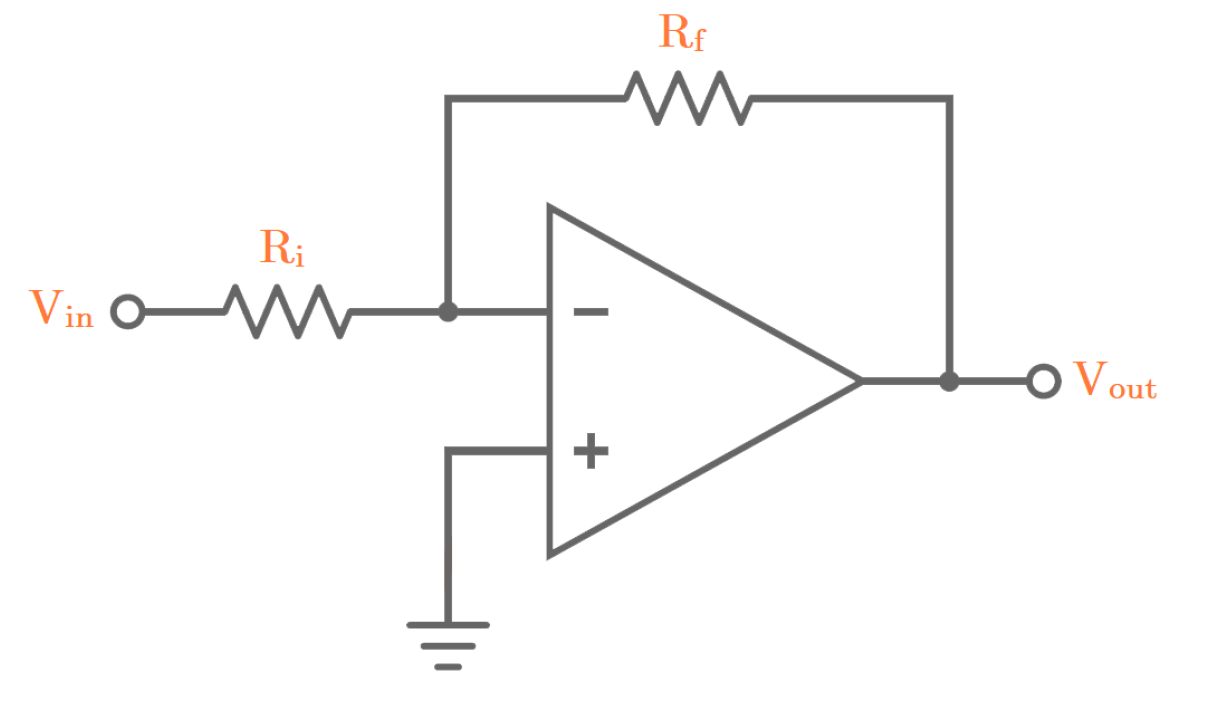
\includegraphics[scale=0.3]{../parte6/Informe_Latex/reources/inverting_opamp_diagram.png}
\caption{Circuito amplificador inversor}
\label{6_invert_opamp_fig}
\end{figure}

\subsubsection{Sumador Ponderado Inversor}
A continuación, en la Figura \ref{6_adder_opamp_fig} se muestra la configuración de un amplificador operacional como sumador ponderado:

\begin{figure}[ht]
\centering
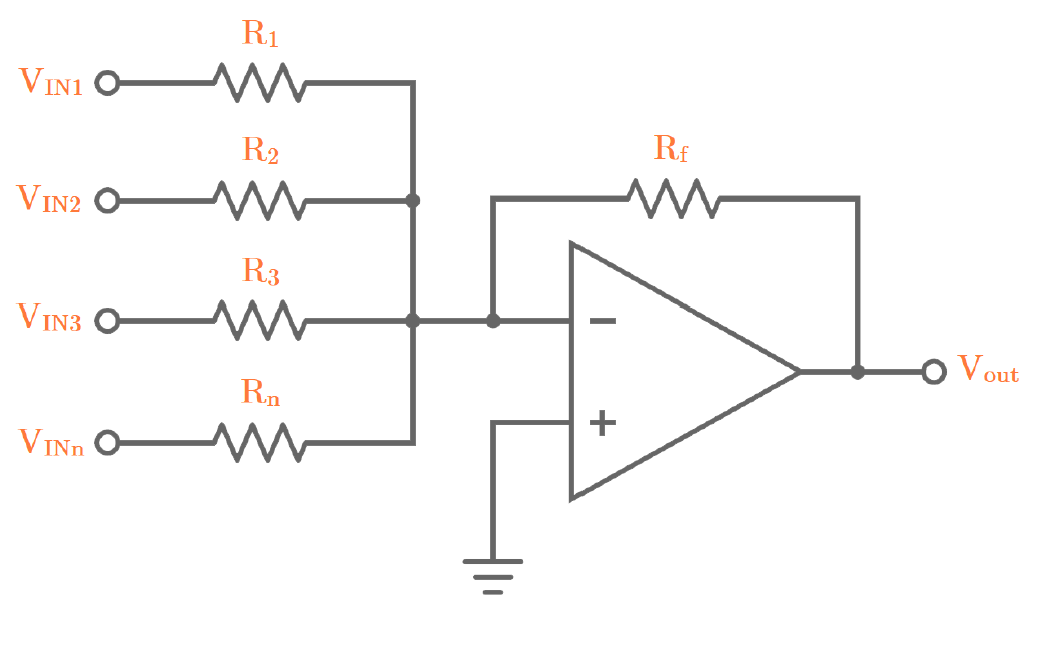
\includegraphics[scale=0.3]{../parte6/Informe_Latex/reources/adder_opamp_diagram.png}
\caption{Circuito amplificador sumador ponderado}
\label{6_adder_opamp_fig}
\end{figure}

La transferencia de este circuito es:
\[\frac{V_{out}}{V_{in}} = - \left(\frac{R_f}{R_1} + \frac{R_f}{R_2} + ... + \frac{R_f}{R_n} \right)\]

\subsection{Disposición y Cálculo de parámetros}
Explicar como se dispusieorn las dos fases anteriores en cascada, resultando en una expresión de $V_{out}$ en función de $V_{in}$ y un offset.
Despejar el valor de esos parametros en funcion de los datos hallados por las condiciones iniciales ($k_1$ y $V_2$).

\section{Implementación en PCB}
Mostrar algo del proceso de diseño (explicar que se hizo extension del circuito para proteger)

\section{Calibración}
Explicar que todas las tolerancias generaban el mismo efecto (offset), por lo que se decidió usar como 'calibrador' al trimmer que setea la $V_{offset}$.

\section{Explicar protección}
Se implementó con Diodos porque son baratos y faciles de poner e intuitivo

\section{Datasheet}
Agregar datos del dispositivo.
